\subsection{Aufgaben}

\begin{enumerate}

 \item Kann man auf Grund des Dominanz\-prinzips bei dem folgenden
 Ent\-scheidungs\-problem bereits feststellen, welche 
Handlungsalternative gewählt werden
sollte oder zumindest sagen, ob eine bestimmte
Handlungsalternative definitiv nicht gewählt werden sollte? 

\begin{center}
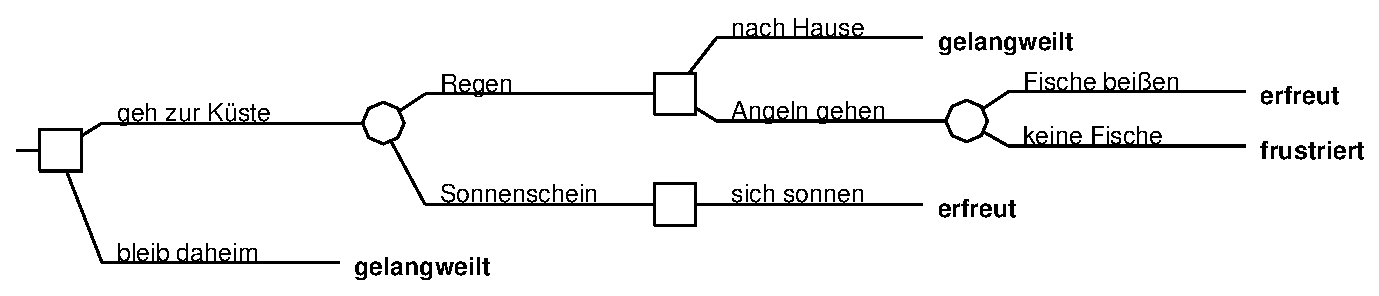
\includegraphics[width=12cm]{Grafiken/Beispiel1_2.eps}
\end{center} 

Erkläutern Sie Ihre
Antwort sowohl anhand der Baum- als auch anhand der Tabellendarstellung (Seite
\pageref{AngelnBeispiel}). Welche Darstellungsform eignet sich dafür besser?

\item Welche Handlungen sollten bei den beiden folgenden Entscheidungs-Tabellen
nach der lexikalischen Maximin-Regel gewählt werden:

\begin{center}
\begin{tabular}{c|c|c|c|c|cc|c|c|c|c|}
\multicolumn{1}{c}{} & \multicolumn{4}{c}{Tabelle 1:} &
\multicolumn{2}{c}{} & \multicolumn{4}{c}{Tabelle 2:}
\\
\cline{2-5} \cline{8-11}
$A_1$ & 1 & -3 & 5   & 6 & & $A_1$ & 0 & 1 & 1 & 3 \\ 
\cline{2-5} \cline{8-11} 
$A_2$ & 2 &  2 & 3   & 3 & & $A_2$ & 0 & 4 & 2 & 3 \\ 
\cline{2-5} \cline{8-11}
$A_3$ & 4 &  6 & -10 & 6 & & $A_3$ & 3 & 0 & 0 & 1 \\ 
\cline{2-5} \cline{8-11}
\end{tabular}

{\tiny Quelle: Michael D. Resnik: Choices. An Introduction to Decision Theory,
Minnesota 2000, S. 27.}
\end{center}

\item Zeige anhand der folgenden Tabelle: Wenn man die lexikalische
Maximin-Regel so abändert, dass der kleinste Wert, sofern er in einer
Zeile mehrmals vorkommt, nicht nur einmal sondern an allen Stellen gestrichen
werden soll, so führt dies dazu, dass durch die lexikalische Maximin-Regel das
Prinzip der Dominanz verletzt werden könnte:

\begin{center}
\begin{tabular}{l|c|c|c|}
\multicolumn{1}{c}{ } & \multicolumn{1}{c}{$S_1$} &
\multicolumn{1}{c}{$S_2$} & \multicolumn{1}{c}{$S_3$}
\\ \cline{2-4}
$A_1$   &    -1  &   2 &  100  \\ \cline{2-4}
$A_2$   &    -1  &  -1 &   3   \\ \cline{2-4}
\end{tabular}
\end{center} 

\item Wie kann man die Maximin-Regel bei Entscheidungsbäumen anwenden?

\item Sei u(x) eine Nutzenskala, die eine Präferenzordnung wiedergibt. Dann gilt:
a) $u(x) > u(y) \Leftrightarrow x \succ y$ und b) $u(x) = u(y) \Leftrightarrow x
\sim y$. {\em Beweise}: Beide Bedingungen gelten auch für die transformierte
Nutzenskala t(u(x)), sofern t der Bedinung für {\em ordinale Transformationen}
genügt: $t(a) > t(b) \Leftrightarrow a > b$ und $t(a) = t(b) \Leftrightarrow a =
b $ für alle a,b auf der Nutzenskala u. 

  ~\\{\bf Schwierigere Aufgabe}\\

\item In der Vorlesung wurde die Präferenzrelation genaugenommen durch zwei
Relationen, nämlich durch die Relation der strikten Präferenz $\succ$ und die
Relation der Indifferenz $\sim$ eingeführt. Zeigen Sie, dass man auch mit einer
einzigen Relation, der schwachen Präferenz $\succeq$ auskommen kann. Geben Sie
dazu geeignete Axiome für die Relation $\succeq$ an. Definieren Sie dann die
Relationen $\succ$ und $\sim$ durch die Relation $\succeq$, und zeigen Sie
anschließend, dass für die so definierten Relationen $\succ$ und $\sim$ die
für sie in der Vorlesung angegeben Axiome gelten.

% \item Für die Olympiade wird eine neue Kombinationssportart aus 5.000m Lauf und
% Weitsprung vorgeschlagen. Für die Beurteilung der Leistungen der Sportler soll
% eine Punktewertung gefunden werden, die so beschaffen ist, dass ein Sportler, der
% im 500m Lauf schneller ist als ein anderer immer auch mehr Punkte bekommt, und
% nur wenn beide Sportler genau gleich gut sind, bekommt derjenige mehr Punkte, der
% im Weitsprung besser abschneidet. Angenommen, die Laufzeiten und die Sprungweiten
% ließen sich unendlich genau messen (m.a.W. es soll angenommen werden, dass die
% Werte reelle Zahlen sind). {\em a) Zeige: Es ist unmöglich eine Punkteskala
% aufzustellen, die beiden Bedingungen genügt.} (Die Moral von dieser Geschichte:
% Nicht alle Arten von wohlgeordneten Präferenzen kann man auf eine lineare
% Nutzenskala abbilden.) {\em b) Zeige weiterhin: Wenn die Messgenauigkeit endlich
% ist, dann ist es sehr wohl möglich eine entsprechende Punkteskala festzulegen.}

% \item Ein Gremium von 5 Personen wird zufällig aus einer Gruppe von 5 Männern und
% 10 Frauen besetzt. Wie groß ist die Wahrscheinlichkeit, dass das Gremium aus 2
% Männern und 3 Frauen besteht? Wie groß ist die Wahrscheinlichkeit, dass das
% Gremium nur aus Frauen besteht?

\end{enumerate}

% \subsection{Zusatzaufgaben}
% 
% \begin{enumerate}
% \item Zeige: Wenn man eine Entscheidungstabelle positiv linear in eine andere
% überführt, dann ist auch die zugehörige Bedauernstabelle eine positiv linear
% transformierte (genaugenommen sogar ein positives Vielfaches, warum?) der
% ursprünglichen Bedauernstabelle. (Was müsste man von der Minimax-Bedauernsregel
% halten, wenn das nicht der Fall wäre?)
% 
% \item Zeige: Positiv lineare Transformationen sind transitiv, d.h. wenn die
% Skala u' durch positiv lineare Transformation aus der Skala u hervorgeht und
% Skala u' durch eine (nicht notwendigerweise dieselbe) positiv lineare
% Transformation in u'' überführt werden kann, dann kann gibt es auch eine
% positiv lineare Transformation, die u unmittelbar in u'' überführt. Warum ist
% diese Eigenschaft wichtig?
% 
% \item Zeige: Jede Entscheidungstabelle kann durch eine positiv lineare
% Transformation in eine Entscheidungstabelle überführt werden, deren maximaler
% Eintrag 1 und deren minimaler Eintrag 0 ist.
% \end{enumerate}

\newpage
